\documentclass{article}

\usepackage{amsmath}
\usepackage{graphicx}
\usepackage{subcaption}
\usepackage{bigfoot}
\usepackage{hyperref}

\title{Project Overview}
\date{5 October 2018}
\author{
	ECE 388
	\\
	\\
	Team 4:
	\\
	Jacob Aubertine
	\\
	Mathieu Bolduc-Clayton
	\\
	Sal Fernandes
}

\begin{document}
	\pagenumbering{gobble}
	\maketitle
	\newpage
	\tableofcontents
	\newpage
	\pagenumbering{arabic}

	\section{Problem Statement}
	Problem statement goes here.

	\section{Description of subsystems}
	Describe subsystems here.
	
	This refers to Figure \ref{fig:oscilloscope}.

	% figure
	\begin{figure}[h!]
		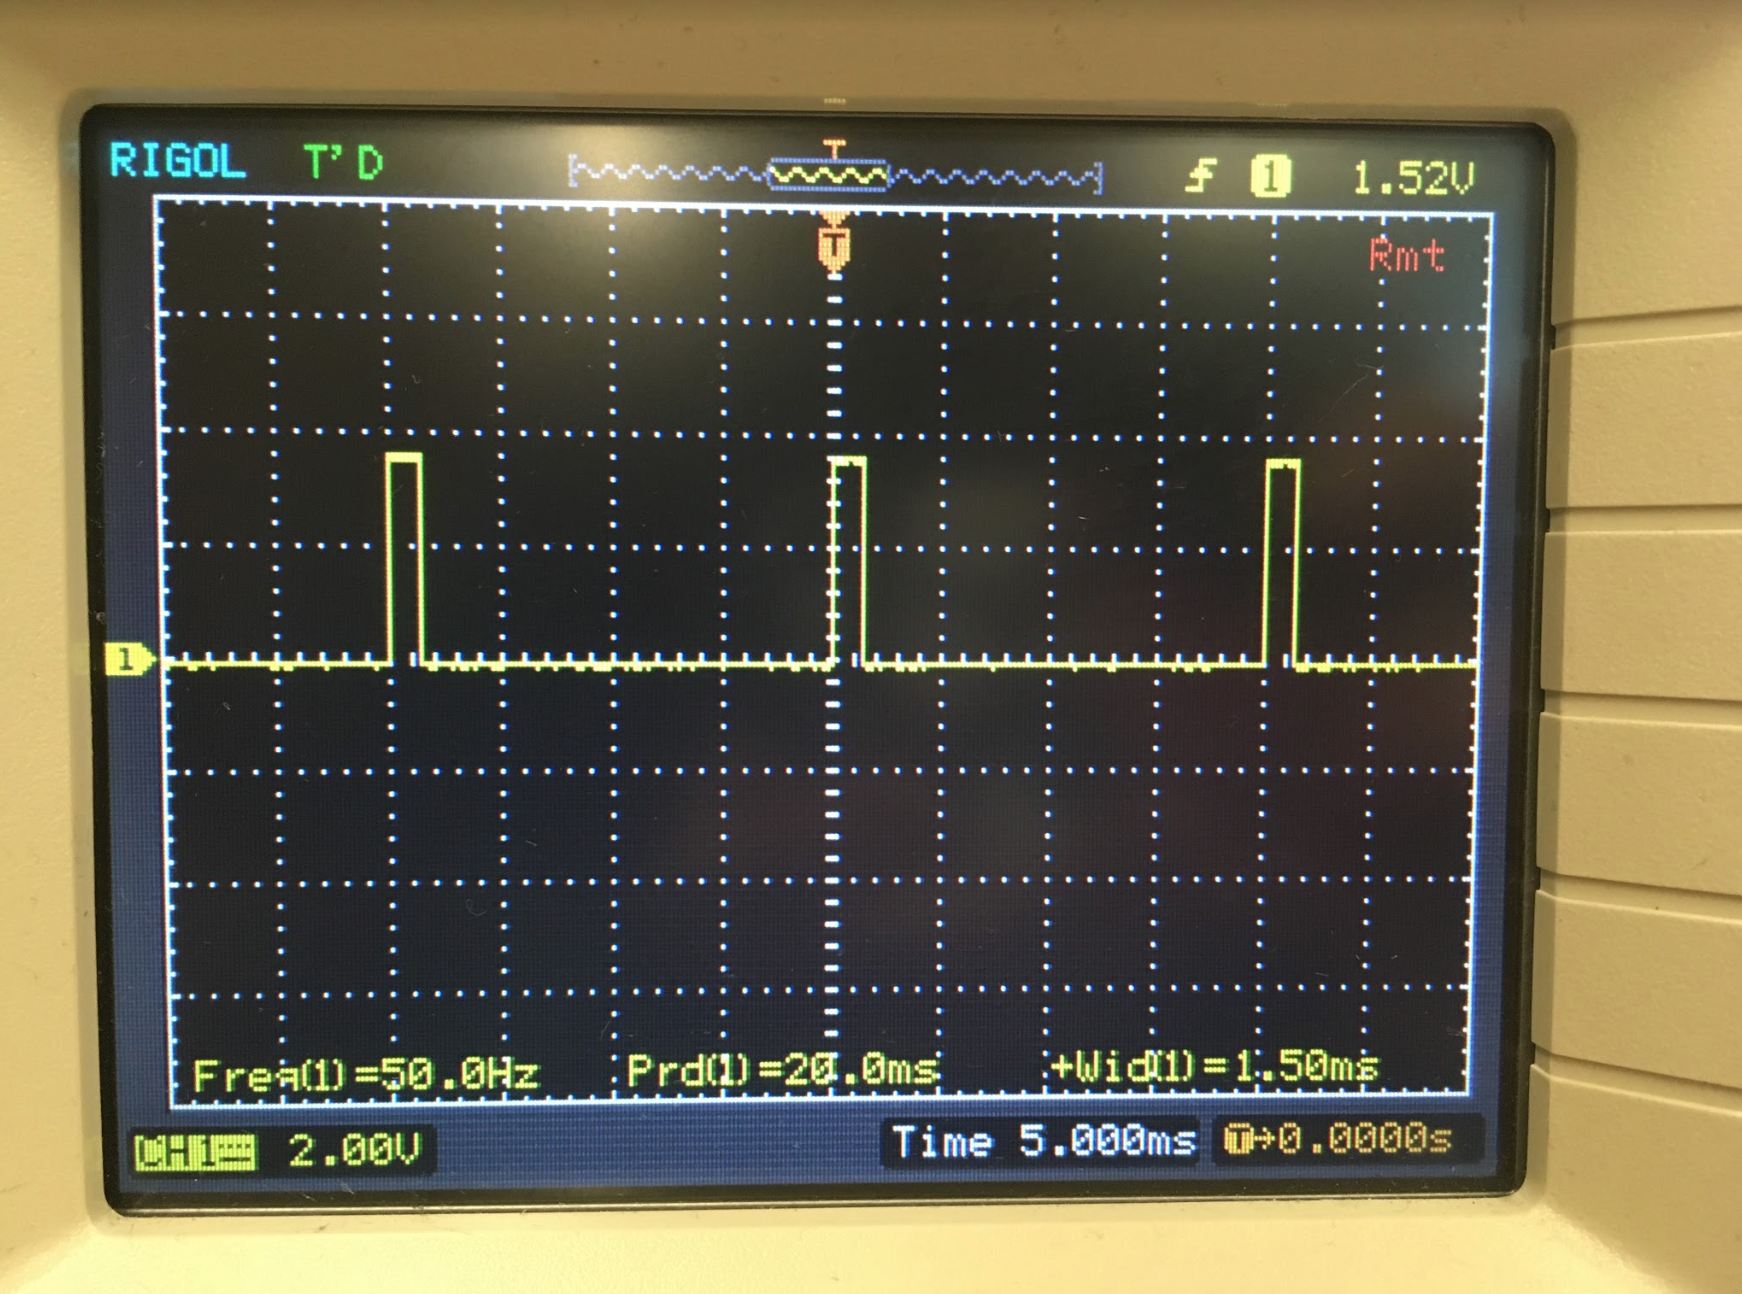
\includegraphics[width=\linewidth]{oscilloscope.png}
		\caption{Oscilloscope readings when connected to function generator.}
		\label{fig:oscilloscope}
	\end{figure}
	
	\section{Work done so far}
	Say what we've done so far.
	
	% table
	\begin{table}[h!]
  		\begin{center}
    			\caption{Team member contributions.}
    			\label{tab:table1}
    			\begin{tabular}{r|r}
      				\textbf{Pulse width} & \textbf{Position (deg)} \\
				\hline
      				1 ms& -90 deg\\
      				1.25 ms & -45 deg\\
      				1.5 ms & 0 deg\\
      				1.75 ms & 45 deg\\
				2 ms& 90 deg\\
   			 \end{tabular}
  		\end{center}
	\end{table}
	
	
	\section{Future test plans}
	Most of the tests specified involve hardware and software working together. Very few tests, at this point, involve just hardware or just software. The subsections are divided roughly by subsystem or component. Since tests often involve multiple subsystems, they are grouped with what was considered most relevant.
	    \subsection{DC motor}
	    \begin{itemize}
            \item When connected to the motor controller, try making the motor rotate in both directions and verify that it does so.
            \item Measure the time it takes for the elevator to travel from the bottom floor to the top, and top floor to the bottom. These times should be the same. Repeat the measurements with different levels of PWM to determine which speed looks most reasonable.
        \end{itemize}
        
	    \subsection{IR distance sensor}
	    \begin{itemize}
	        \item The sensor by itself had been tested by using a voltmeter to measure its voltage at specfic distances.
	        \item After connecting the sensor to the microcontroller ADC, test the readings at different distances.
	        \item Record the readings again, this time with the sensor at the top of the elevator shaft. Get positions for each floor based on the distance from the sensor.
	        \item Once the positions are known, have the elevator travel to each floor from above and below (if possible) to measure how far the elevator is physically from the desired position. The elevator should line up from both directions.
	        \item Set a distance for the motor to stop at, and see how long it takes for it to stop, and record how far it stopped from the desired location.
	    \end{itemize}
	    
	    \subsection{Buzzer}
	    \begin{itemize}
	        \item Send the elevator to a floor and verify that the buzzer buzzes when it reaches the floor.
	        \item Press the emergency stop button, verify that the buzzer buzzes until the button is pressed again.
	    \end{itemize}
	    
	    \subsection{Emergency stop}
	    \begin{itemize}
	        \item Press emergency stop to stop elevator. Try to press buttons to call elevator and send it to another floor. The elevator should not move until the emergency stop is disengaged.
	    \end{itemize}
	    
	    \subsection{Security: magnetic stripe reader}
	    \begin{itemize}
	        \item With the reader connected to the microcontroller, record the data received from swiping a card. This card and its data will be considered valid. Try to get a match by swiping other cards. Ideally they should not match and should be rejected.
	        \item The elevator should not be called until a valid card is swiped. Try different input combinations to move elevator or open a door before a valid card is swiped. Also try this when an invalid card is swiped. Repeat the same tests by swiping a valid card and ensure that the doors open and the elevator does move (if not on the floor).
	    \end{itemize}
	    
	    \subsection{Door}
	    \begin{itemize}
	        \item The door should open shortly after a floor is reached. This time will be measured and adjusted as necessary, and must be after the elevator stops moving.
	        \item The door should then close some time after a floor is reached and remained closed until a valid card is swiped. This time will also be measured and adjusted to ensure passengers have enough time to safely exit the elevator.
	        \item The door should remain closed while moving, and the elevator should continue to its destination before moving to another floor. The call buttons should be pressed for different floors while the elevator is moving to make sure it continues and the doors remain closed until stopped.
	        \item If at a floor with the door open and something is detecting in the path of the door, the door should remain open and the elevator should not move until the path is clear for a time. The call buttons should be pressed while the path is blocked to test if the elevator does actually move. The time it takes the door to close after the path has been cleared will be measured to ensure it can safely be cleared and remain clear.
	    \end{itemize}
	    
	    \subsection{Buttons}
	    \begin{itemize}
	        \item The button matrix should be tested independently to ensure every button can be properly detected.
	        \item The emergency stop button should halt all function and continue to until it is pressed again. This should be tested when the elevator is in different positions, such as when it is moving between floors and stopped at a floor.
	    \end{itemize}
        
\end{document}